\chapter{Dispersed phase simulation in BIMER}
	\label{ch9:BIMER_lagrangian}

\section{Introduction}

The previous chapter has reported the resolved atomization simulations performed through one multipoint injector of the BIMER configuration. The lagrangian injector learning process was applied to get a in-plane, spatially distributed spray. This spray conforms a lagrangian injector that is used in this chapter to initialize the liquid phase dispersed-phase simulations. The dense core was also characterized: these information can be used in this chapter to impose an actuator with the ALM method that perturbs the gaseous phase similarly to a jet dense column. Due to rotational symmetry in the multipoint stage, the obtained SLI and actuator can be extrapolated to the remaining multipoint holes to perform liquid injection and gaseous phase perturbation in the full configuration. This chapter reports the results of \hl{one (two?)} dispersed-phase simulation\hl{(s)} of BIMER with the SLI methodology.

In first place, the computational setup is explained in $\S$\ref{ch9:sec_computations_setup}. The multipoint injection is briefly detailed here, while the pilot injection performed with the LISA injection model is thoroughly explained. Then, available experimental results for this configuration and the operating point chosen, which can be used for computational validation, obtained by \citeColor[renaud_high-speed_2015] are summarized in $\S$\ref{ch9:sec_expe_results_LGS_BIMER}. The SLI flowchart, which was generally detailed in Figure \ref{fig:SLI_graphic_description} for a JICF, is extended to BIMER in $\S$\ref{sec:ch9_BIMER_SLI_flowchart}. Next, the SLI used for lagrangian injector and the effect of the proposed ALM in the gaseous field are reported in $\S$\ref{sec:ch9_BIMER_BCs_for_phases}. Finally, the results from \hl{one (two)}  simulation\hl{(s)} are reported and discussed in $\S$\hl{\textbf{XX}}. \hl{It is shown that ...}





\section{Computational setup}
\label{ch9:sec_computations_setup}


For performing dispersed phase simulations, the operating point defined in Table \ref{tab:liquid_operating_point_Renaud} is simulated. The staging factor is $\alpha = 15$, meaning that $15 \%$ of the total liquid flow rate is injected through the pilot stage and the remaining liquid through the multipoint. For total flow rate of $\dot{m}_l = 1.64$ g s$^{-1}$, the take-off stage injects a mass flow rate of $\dot{m}_{l,takeoff}$ = 1.39 g s$^{-1}$ (hence $0.139$ g s$^{-1}$, corresponding to $Q_l = 185.3$ mm$^3$s$^{-1}$,  per injector), and a mass flow rate of $\dot{m}_{l,p} = 0.25$ g s$^{-1}$ is introduced through the pilot stage. The global equivalence ratio of this operating point is $\phi_g = 0.6$.

\subsubsection*{Evaporation}

Due to the high gas ambient temperature inside BIMER combustion chamber, evaporation of lagrangian droplets should be considered. In this case ...

%\begin{table}[!h]
%\centering
%\caption{Operating point to perform gaseous and two-phase simulations tested by \citeColor[renaud_high-speed_2015]}
%\begin{tabular}{|c|c|c|c|}
%\hline
%\multicolumn{4}{|c|}{\textbf{Air properties}} \\
%\hline
%$\dot{m}_g$ [g s$^{-1}$] & $T_g$ [K] & $\rho_g$ [kg m$^{-3}$]  & $\mu_g$ [Pa s]  \\
%\hline
%43.1 & 433 & 0.816382 & $2.3911 \cdot 10^{-5}$ \\
%\hline
%\hline
%\multicolumn{4}{|c|}{\textbf{Liquid properties}} \\
%\hline
%$\dot{m}_l$ [g s$^{-1}$] & $\rho_l$ [kg m$^{-3}]$   & $\mu_l$ [Pa s]   & $\sigma$ [N m$^{-1}$]   \\
%\hline
%1.64 & 750 & $1.36 \cdot 10^{-3}$ & $25.35 \cdot 10^{-3}$ \\
%\hline
%\hline
%\multicolumn{4}{|c|}{\textbf{Burner staging}} \\
%\hline
%$\alpha$ [$\%$] &  $\dot{m}_{l,p}$ [g s$^{-1}$] & $\dot{m}_{l,t}$ [g s$^{-1}$] & $\phi_g$ [-]\\
%\hline
%15 & 0.25 & 1.39 & 0.6 \\
%\hline
%\end{tabular}
%\label{tab:liquid_operating_point_Renaud}
%\end{table}

\clearpage


\begin{table}[!h]
\centering
\caption{Operating point to perform gaseous and two-phase simulations tested by \citeColor[renaud_high-speed_2015]}
\begin{tabular}{cccc}
\thickhline
\multicolumn{4}{c}{\textbf{Air properties}} \\
\hline
$\dot{m}_g$ [g s$^{-1}$] & $T_g$ [K] & $\rho_g$ [kg m$^{-3}$]  & $\mu_g$ [Pa s]  \\
\hline
43.1 & 433 & 0.82 & $2.4 \cdot 10^{-5}$ \\[0.075in] %0.816382 & $2.3911 \cdot 10^{-5}$ \\[0.075in]
%%\bottomrule
%\\[0.1in]
%%\vspace*{0.1in}
\thickhline
\multicolumn{4}{c}{\textbf{Liquid properties}} \\
\hline
$\dot{m}_l$ [g s$^{-1}$] & $\rho_l$ [kg m$^{-3}]$   & $\mu_l$ [Pa s]   & $\sigma$ [N m$^{-1}$]   \\
\hline
1.64 & 750 & $1.36 \cdot 10^{-3}$ & $25 \cdot 10^{-3}$ \\[0.075in] %25.35 
\thickhline
\multicolumn{4}{c}{\textbf{Burner staging}} \\
\hline
$\alpha$ [$\%$] &  $\dot{m}_{l,pilot}$ [g s$^{-1}$] & $\dot{m}_{l,takeoff}$ [g s$^{-1}$] & $\phi_g$ [-]\\
\hline
15 & 0.25 & 1.39 & 0.6 \\
\thickhline
\end{tabular}
\label{tab:liquid_operating_point_Renaud}
\end{table}

%\begin{table}[!h]
%\centering
%\caption{Operating point to perform gaseous and two-phase simulations tested by \citeColor[renaud_high-speed_2015]}
%\begin{tabular}{cccc}
%\thickhline
%\multicolumn{4}{c}{\textbf{Air properties}} \\
%\thickhline
%$\dot{m}_g$ [g s$^{-1}$] & $T_g$ [K] & $\rho_g$ [kg m$^{-3}$]  & $\mu_g$ [Pa s]  \\
%\hline
%43.1 & 433 & 0.816382 & $2.3911 \cdot 10^{-5}$ \\
%\end{tabular} \\
%\medskip
%\begin{tabular}{cccc}
%\thickhline
%\multicolumn{4}{c}{\textbf{Liquid properties}} \\
%\hline
%$\dot{m}_l$ [g s$^{-1}$] & $\rho_l$ [kg m$^{-3}]$   & $\mu_l$ [Pa s]   & $\sigma$ [N m$^{-1}$]   \\
%\hline
%1.64 & 750 & $1.36 \cdot 10^{-3}$ & $25.35 \cdot 10^{-3}$ \\
%\end{tabular} \\
%\medskip
%\begin{tabular}{cccc}
%\thickhline
%\multicolumn{4}{c}{\textbf{Burner staging}} \\
%\hline
%$\alpha$ [$\%$] &  $\dot{m}_{l,p}$ [g s$^{-1}$] & $\dot{m}_{l,t}$ [g s$^{-1}$] & $\phi_g$ [-]\\
%\hline
%15 & 0.25 & 1.39 & 0.6 \\
%\hline
%\end{tabular}
%\label{tab:liquid_operating_point_Renaud}
%\end{table}





\section{Experimental results from literature}
\label{ch9:sec_expe_results_LGS_BIMER}

The BIMER operating point tested in this chapter to test the SLI methodology has been chosen since it presents non-reactive experimental results that can be used for validation. These ones, shown in the PhD thesis of \citeColor[renaud_high-speed_2015], consist of the qualitative maps of SMD, axial and vertical velocities shown in Figure \ref{fig:maps_BIMER_renaud_expe_results}. Qualitative experimental results on non-reactive conditions are not available from literature, and hence a qualitative validation is not possible to this date.

\begin{figure}[h!]
\flushleft
\begin{subfigure}[b]{0.3\textwidth}
	\centering
   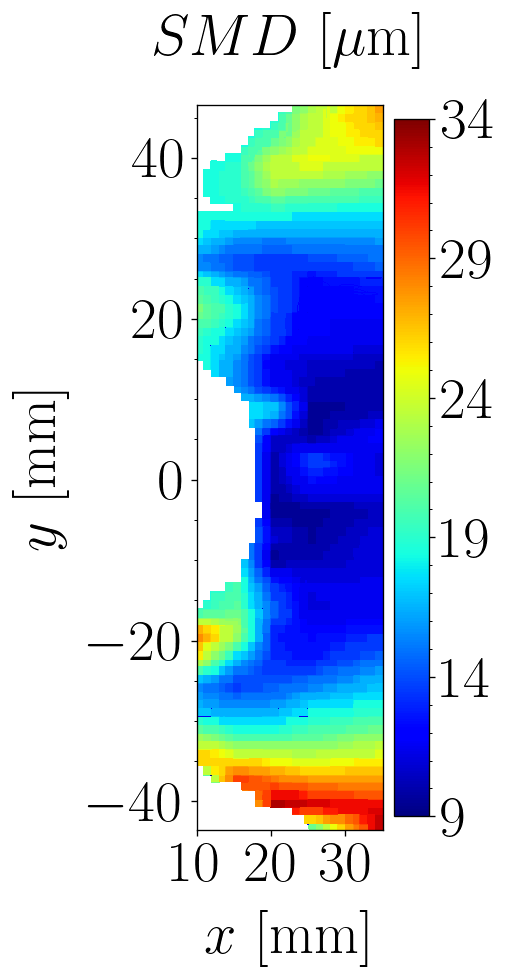
\includegraphics[scale=0.4]{./part3_applications/figures_ch9_lagrangian/expe_maps/SMD_map.png}
   %\caption{Low Weber number operating point.}
   %\label{} 
\end{subfigure}
\hspace*{0.1in}
\begin{subfigure}[b]{0.3\textwidth}
	\centering
   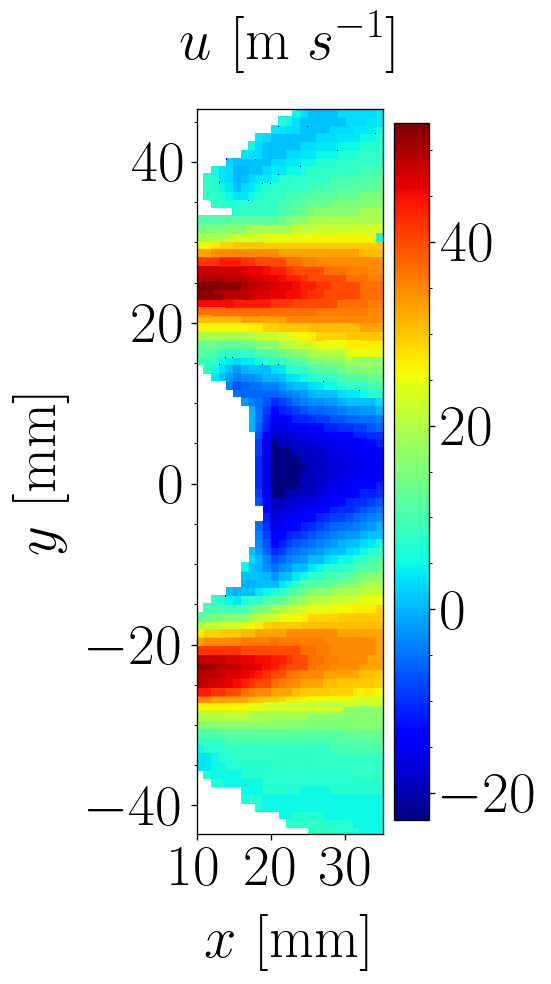
\includegraphics[scale=0.4]{./part3_applications/figures_ch9_lagrangian/expe_maps/u_axial_map.png}
   %\caption{Low Weber number operating point.}
   %\label{} 
\end{subfigure}
\hspace*{0.1in}
\begin{subfigure}[b]{0.3\textwidth}
	\centering
   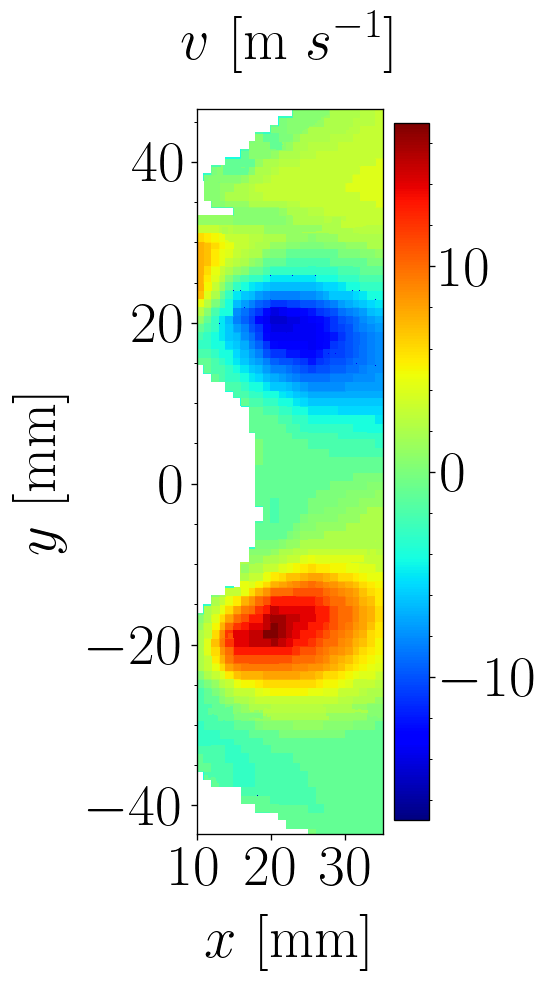
\includegraphics[scale=0.4]{./part3_applications/figures_ch9_lagrangian/expe_maps/u_vertical_map.png}
   %\caption{Low Weber number operating point.}
   %\label{} 
\end{subfigure}
\caption{Experimental maps for for $SMD$, axial velocity $u$ and vertical velocity $v$ from \citeColor[renaud_high-speed_2015]}
\label{fig:maps_BIMER_renaud_expe_results}
\end{figure}

%\section{Model flowchart applied to BIMER}
%\label{sec:ch9_BIMER_SLI_flowchart}

\section{Boundary condition for liquid phase}
\label{sec:ch9_BIMER_BCs_for_liquid_phase}


\subsection{Multipoint stage injection}

For the multipoint stage, the SLI obtained from the resolved atomization simulations in Chapter \ref{ch8:bimer_resolved_atomization} are used. Since the objective of this simulation is to prove that SLI can be used to initialise dispersed-phase computations in a full multipoint injector, only the SLI obtained from the fine simulation with $\Delta x_\mathrm{min} = 10~\mu$m at the location $x_c = 2$ mm is used. This injector is chosen since 1) it has been obtained with the finest interface resolution simulated and 2) it has been obtained at an axial location along the crossflow direction $x_c$ where all the global spray mean magnitudes (SMD, velocities, deformation parameters) are converged with axial distance (see $\S$\ref{sec:ch8_BIMER_spray_char}). This SLI is shown in Figure \ref{fig:injectors_sli_BIMER_DX10_xD06p67}: these maps, \hl{with(out) convergence-driven discretization}, are injected as shown in the dispersed phase simulation. The flux spatial distribution in the SLI is scaled so that the total mass flow rate injected in one multipoint hole is equal to the actual mass flow rate injected in the experimental configuration. Injected velocities are \hl{volume-weighted/artimethci mean} and RMS following a gaussian $r$ velocity law. The secondary atomization model chosen is the Gorokhovski model with constants $K_1 = $\textbf{XX?}, $K_2 = $\textbf{XX?}. These injection parameters are summarized in Table  \ref{tab:BIMER_SLI_fixed_model_parameters}.


\begin{table}[!h]
\centering
\caption{Fixed SLI model parameters for dispersed-phase simulations of the take-off stage in BIMER}
\begin{tabular}{cccccc}
\thickhline
 \multirow{2}{*}{ \begin{tabular}{c} \textbf{Resolved} \\ \textbf{simulation} \end{tabular}}    &  \multirow{2}{*}{  \begin{tabular}{c} $x_{c,\mathrm{inj}}$  \\ $\left[ \mathrm{mm} \right]$ \end{tabular}} &   \multirow{2}{*}{ \begin{tabular}{c} $\textbf{r}$ \\ \textbf{law} \end{tabular}} & \multirow{2}{*}{ \begin{tabular}{c} \textbf{Atomization} \\ \textbf{model} \end{tabular}} &    \multirow{2}{*}{ $K_1$} & \multirow{2}{*}{ $K_2$}\\
 & & & & &  \\
\thickhline
DX10 & 2 & Gaussian & Goro  & ? & ? \\
\thickhline
\end{tabular}
\label{tab:BIMER_SLI_fixed_model_parameters}
\end{table}


For performing injection in the 10 multipoint holes, the SLI from the single liquid injector simulated are replicated in the remaining liquid injectors. For it, the injectors location are translated and the vectorial magnitudes (crossflow normal direction, velocities) are rotated so that the crossflow local direction stays identical in all multipoint holes. Each single injector will deliver a mass flow rate of $\dot{m}_{l,t} = 0.139$ g s$^{-1}$ (equivalent to a flow rate of $Q_l = 185.3$ mm$^3$ s$^{-1}$), hence making a total liquid flux injected of $\dot{m}_{l,t} = 1.39$ g s$^{-1}$ for the take-off phase as indicated in Table \ref{tab:liquid_operating_point_Renaud}. A schematic view of three injectors through which lagrangian droplets will be injected can be seen in Figure \ref{fig:BIMER_multipoint_injection_planes_view}.

%These injectors were, however, obtained from the simulations of one single injector. In order to initialise the rest of multipoint injection holes (for a total of 10 in BIMER, see Figure \textbf{Figure??}), new numerical injectors need to be defined in each hole by making a revolution of the available ones. This revolution is possible due to the radial of BIMER in terms of injectors location (which are equally spaced to a distance of 25 mm from the center with a radial difference of 36 $\degree$) and the multipoint vane locations: each injection hole is located at the same location between two vanes, hence seeing the same incoming air (see Figure \textbf{Figure??}).

\begin{figure}[h!]
	\centering	\includeinkscape[inkscapelatex=false,scale=0.5]{./part3_applications/figures_ch9_lagrangian/multipoint_injection_planes_view}
	\caption{View of BIMER take-off stage showing three different injection locations}	\label{fig:BIMER_multipoint_injection_planes_view}
\end{figure}





\subsection{Pilot stage injection}

The operating point simulated injects fuel through both a take-off stage (which has been modelled with the SLI) and a pilot stage. Since pilot stage has not been simulated with the methodology developed in this thesis, another approach must be employed. Given that the pilot of BIMER injects fuel following a hollow cone configuration, the LISA model introduced in $\S$\ref{subsec:ch3_hollow_cone_spray} will be used \citepColor[guedot_developpement_2015].   The input parameters for the LISA model to inject a hollow cone spray are summarized in Table \ref{tab:LISA_model_parameters}. For the mean opening angle, a value $\theta_s = 30 \degree$ is taken from experiments \citepColor[renaud_high-speed_2015]. Regarding the droplet's diameter, previous studies using lagrangian approaches on the same configuration have introduced directly droplets size distributions extracted from experimental data \citepColor[mesquita_large_2018]. In this case, since for the operating condition simulated there is not experimental size distributions available, droplets injected will have a constant diameter given by the following experimental correlation \citepColor[lefebvre_atomization_2017]:

\begin{equation}
SMD = 2.25 \left( \sigma \dot{m}_f \mu_l \right)^{0.25} \rho_g^{-0.25}  \Delta P^{-0.5}
\end{equation}

where $\Delta P = 2.6$ MPa is the pressure drop in the pilot nozzle \citeColor[renaud_high-speed_2015]. Applying the previous correlation with the magnitudes given in Table \ref{tab:liquid_operating_point_Renaud} results in a diameter $SMD = 15~\mu$m imposed to the pilot cones particles. Such particles will later break due to the action of the secondary atomization model. The breakup model is constant in all the simulations and therefore is identical for both the take-off and pilot stages, hence the Gorokhovski model with the constants defined in Table \ref{tab:BIMER_SLI_fixed_model_parameters} is applied to the pilot droplets. 

 %this correlation provides a SMD of $15 \mu m$ (\textbf{CHECK THIS}).

% dP value is tiven in Renaud p. 24, or 46 PDF

\begin{table}[!h]
\centering
\caption{LISA model setup for pilot injection}
\begin{tabular}{ccc}
\thickhline
\textbf{Parameter} & \textbf{Units} &  \textbf{Value} \\
\thickhline
Mass flow rate $\dot{m}$ & g s$^{-1}$ & 0.25 \\
%\hline
Injector radius $R_0$ & mm & 0.125 \\
%\hline
Mean angle $\overline{\theta}_s$ & $\degree$ & 30  \\
SMD & $\mu$m & 15 \\
\thickhline
\end{tabular}
\label{tab:LISA_model_parameters}
\end{table}

\subsubsection*{LISA model for injection (REMOVE WHEN SIMUS READY)}

For performing pilot injection, the LISA model available in YALES2 is used \citepColor[guedot_developpement_2015]. 

\begin{equation}
X = \frac{A_a}{A_0} = \left( \frac{R_a}{R_0} \right)^2 = \frac{\sin^2 \gamma_s}{1 + \cos^2 \gamma_s}
\end{equation}

where $R_a$ is the minimum injection radius, $R_0$ the maximum, and $\gamma_s$ is the mean injection angle. The inputs to the model are $\gamma_s$ and $R_0$, so from the previous equation $X$ can be obtained and the radius $R_a$ can be solved:

\begin{equation}
R_a^2 = R_0^2 X
\end{equation}

The axial velocity imposed to the particles $u_x$ is obtained through the following expression:

\begin{equation}
u_x = \frac{\dot{m}}{\rho_l \pi \left( R_0^2 - R_a^2 \right)} = \frac{\dot{m}}{\rho_l \pi R_0^2 \left( 1 - X^2 \right)} 
\end{equation}

\textbf{OJO}: in Renaud's application case ($\dot{m} = 0.25 ~ g/s$, see Table \ref{tab:LISA_model_parameters}), taking $R_0 = 0.125 ~mm$ gives an axial velocity of $u_x = 7.9 ~ m/s$. This created an almost-point injection, as it can be seen in the simulations. If we take $R_0 = 1.5 ~mm$ (the radius of the hollow cone patch), droplets are injected along all the hollow cone patch. However, the axial velocity imposed is $u_x = 0.05 ~m/s$. So we'll go towards the large radius.

%\begin{table}[!h]
%\centering
%\caption{LISA model setup for pilot injection}
%\begin{tabular}{|c|c|}
%\hline
%\textbf{Parameter} & \textbf{Value} \\
%\hline
%Mass flow rate $\dot{m} [g s^{-1}]$ & 0.25 \\
%\hline
%Injector radius $R_0 [mm]$ & 0.125 \\
%\hline
%Mean angle $\overline{\theta} [\degree]$ & 40 \\
%\hline
%\end{tabular}
%\label{tab:LISA_model_parameters}
%\end{table}




\section{Boundary condition for gaseous phase}
\label{sec:ch9_BIMER_BCs_for_gaseous_phase}

The perturbation effect of the liquid dense core, which is be directly accounted for by the lagrangian droplets, can also be modelled in BIMER. In this case, the direct prescription of a perturbed gaseous inlet in a reduced domain as described in $\S$\ref{subsec:ch6_jicf_lgs_gaseous_inlet_prescription} cannot be performed \hl{due to the complexity of the multi-staged injector}. Therefore, only the ALM methodology ($\S$\ref{sec:ch4_dense_core_modelling}) is applied for this purpose. In a first step, the input parameters to the model are taken from the results of the resolved atomization simulation DX10: dense core topology from the results shown in Figure \ref{fig:BIMER_DC_mean_parameters_scatterplots} and net force from Table \ref{tab:BIMER_dense_core_pressures_and_force_parameters}.  These parameters are referred as the initial ones in Table \ref{tab:BIMER_lgs_ALM_parameters}. As for the ALM model applied to the traditional JICF in $\S$\ref{sec:ch6_BC_gaseous_phase}, these initial parameters have been found not to accurate capture the actual momentum exchange between the gas and the liquid in the resolved simulation, and are hence tuned to find a better match between the turbulent gaseous structures in the resolved and dispersed-phase computations. The final parameters obtained are shown in the corresponding column of Table \ref{tab:BIMER_lgs_ALM_parameters}. In this chapter, only the final ALM parameters will be tested in dispersed-phase simulations.

\begin{table}[!h]
\centering
\caption{Parameters of an actuator representing the BIMER dense core}
\begin{tabular}{cccc}
\thickhline
\textbf{Parameter} & \textbf{Units} & \textbf{Initial} &  \textbf{Final} \\
\thickhline
$x_b$ & mm & 0.34 & 0 \\
$z_b$ & mm & 1.43 &  \\
%$c_0$ & mm & 0.3  & 0.3 \\
%$c_L$ & mm & 0.35 & \\
$| \textbf{F}_\mathrm{DC} |$ & N & 0.25 $\cdot 10 ^{-3}$ & 0.8 \\
%$\Delta p$ & Pa &  & \\
\thickhline
\end{tabular}
\label{tab:BIMER_lgs_ALM_parameters}
\end{table}

%\subsection{Effect of dense core perturbation}

%\subsection{Effect of evaporation}

\section{Simulations and results}

Three dispersed-phase simulations are performed for the BIMER configuration. All of them use the same boundary conditions for the liquid phases in the take-off (SLI model) and the pilot (LISA model) stages. They differ in the inclusion of the perturbation effect in the gaseous phase through ALM and the consideration of evaporation. A baseline simulation is performed without neither ALM nor evaporation. Then, both contributions are studied separately in two distinct simulations. The computations performed are summarized in Table \ref{tab:BIMER_dispersed_phase_simulations_performed}.

\begin{table}[!h]
\centering
\caption{Dispersed-phase simulations performed for BIMER}
\begin{tabular}{ccc}
\thickhline
\textbf{Case} & \textbf{ALM} & \textbf{Evaporation} \\
\thickhline
Baseline & No & No \\
ALM & \textcolor{blue}{Yes} & No \\
Evap & No & \textcolor{blue}{Yes} \\
\thickhline
\end{tabular}
\label{tab:BIMER_dispersed_phase_simulations_performed}
\end{table}


\subsubsection*{Characteristic liquid times}

As in the resolved atomization simulations of one multipoint injector, characteristic liquid times can be defined for the liquid phase in the dispersed-phase computations. The interest here is to relate the physical simulation time to a characteristic time scale related to the magnitudes to be studied. In this case, these magnitudes are the SMD and droplets velocities in the spatial region downstream the combustion chamber where experimental PDA results have been obtained (Figure \ref{fig:maps_BIMER_renaud_expe_results}). Since this region spans up to a downstream location $x = 35$ mm, the characteristic time will be defined as the time that the first droplet takes to reach this axial coordinate from the beginning of the simulation: $\tau_{\mathrm{dr}_{x=35\mathrm{mm}}}$. Therefore, the dimensionless simulated time $t^{\prime}$ is defined according to Eq. (\ref{eq:t_prime_BIMER_LGS}):

\begin{equation}
\label{eq:t_prime_BIMER_LGS}
t^{\prime} = t / \tau_{\mathrm{dr}_{x=35\mathrm{mm}}}
\end{equation}


Table \ref{tab:BIMER_dispersed_phase_characteristic_times}.  summarized the characteristic times obtained in the simulations performed. As observed in this table, the characteristic times chosen are of the order of the gaseous swirl time scale $\tau_\mathrm{swirl}$ for this operating point (Table \ref{tab:gaseous_field_timescales}) while they differ of one order of magnitude with respect to the liquid characteristic times of the resolved atomization simulations (see Tables \ref{tab:BIMER_SPS_characteristic times} and \ref{tab:BIMER_SPS_characteristic_droplet_sampling_times}).  This shows again (this was also demonstrated in the lagrangian simulations of Chapter \ref{ch6:jicf_lgs_simulations}) how the dispersed phase computations allow to simulate more physical times and obtain converged spray fields with less computational time than the resolved atomization simulations. 


\begin{table}[!h]
\centering
\caption{Characteristic times for droplets to reach location $x = 35$ mm in the pilot and take-off stages }
\begin{tabular}{ccc}
\thickhline
\textbf{Case} & $\tau_{\mathrm{dr}_\mathrm{pilot}}$ [ms] & $\tau_{\mathrm{dr}_\mathrm{takeoff}}$ [ms] \\
\thickhline
Baseline & 1.65 & 2.45 \\  % restart_01, it. 330 ; restart_01, it. XX
ALM & 1.52 & 2.32 \\ % restart_02, it. 143
Evap & 1.48 & 2.25 \\ % restart_01, it. 295
\thickhline
\end{tabular}
\label{tab:BIMER_dispersed_phase_characteristic_times}
\end{table}





\subsection{Spray flow field}

\subsection{Qualitative results and experimental comparison}

\clearpage

\begin{figure}[h!]
\centering
\begin{subfigure}[b]{1.0\textwidth}
	\centering 
	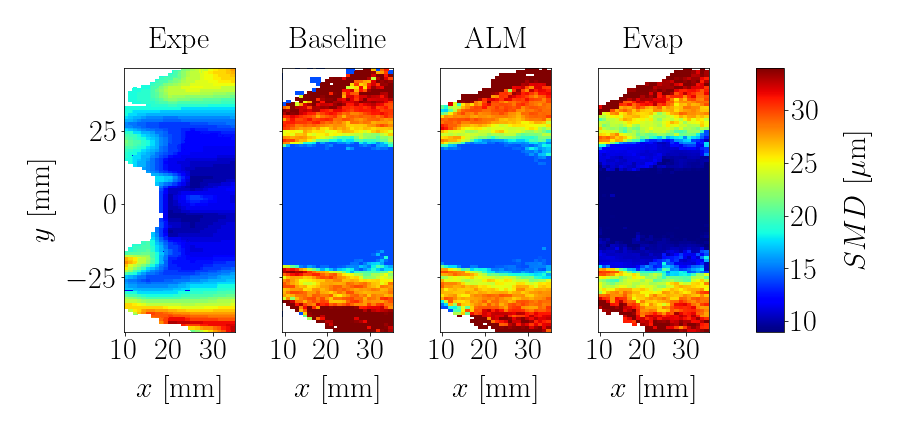
\includegraphics[scale=0.4]{./part3_applications/figures_ch9_lagrangian/simus_expe_validation/subplots_maps_SMD.png}
   \caption{SMD maps}
   %\label{fig:validation_qualitative_u_mean} 
\end{subfigure}

\vspace*{0.1in}

\begin{subfigure}[b]{1.0\textwidth}
	\centering
	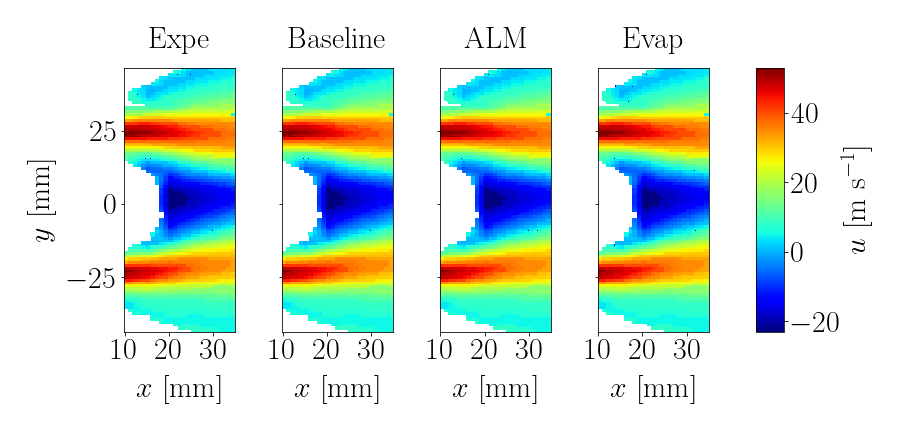
\includegraphics[scale=0.4]{./part3_applications/figures_ch9_lagrangian/simus_expe_validation/subplots_maps_axial_velocity.png}
   \caption{Mean axial velocity maps}
   %\label{fig:validation_qualitative_u_rms}
\end{subfigure}

\vspace*{0.1in}

\begin{subfigure}[b]{1.0\textwidth}
	\centering
	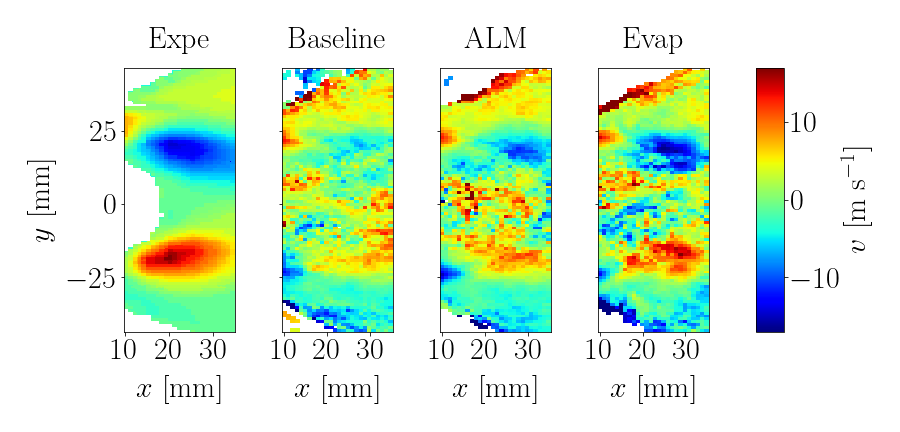
\includegraphics[scale=0.4]{./part3_applications/figures_ch9_lagrangian/simus_expe_validation/subplots_maps_vertical_velocity.png}
   \caption{Mean vertical velocity maps}
   %\label{fig:validation_qualitative_v_mean} 
\end{subfigure}
\caption[Qualitative experimental validation]{Qualitative experimental validation in the region enclosed in Figure \textbf{XX?}. SMD, mean and vertical velocity fields velocity from experiments by \citeColor[renaud_high-speed_2015] and the three simulations performed}
\label{fig:validation_BIMER_lgs}
\end{figure}

\clearpage

\section{Computational performances}

\section{Conclusions}


This chapter has shown the application of SLI to initialize the dispersed liquid phase in the academic multipoint injector BIMER. The methodology has been applied to the take-off stage by using the SLI constructued from the resolved atomization simulations of Chapter \ref{ch8:bimer_resolved_atomization}. The SLI obtained from one injection hole has been extrapolated to the rest of the multipoint to initialize the liquid phase in all the take-off stage. This has been possible thanks to the symmetry of the multipoint injector. The pilot stage, which produces a hollow cone-type injection, has been approximated with the LISA 
model. For the gaseous phase, the ALM methodology has been applied to model the perturbation of the BIMER dense core in the aerodynamic field. As in the SLI, the perturbation effect has been studied in the resolved simulations for one injection hole and then extrapolated to the rest of injectors in the dispersed-phase simulation. To study the influence of the ALM, one simulation has been without perturbing the gaseous phase at the vicinity of the injectors by taking as initial conditions the simulation from Chapter \ref{ch7:bimer_test_bench_and_aero}. \hl{Additionally, evaporation has also been included in a third simulation to better replicate the multiphysics conditions found within these injectors, since ambient temperature in the operating point studied is high enough for evaporation to take place.}

\hl{We also need to specify that the initial conditions for ALM extracted from the resolved simulations are not so useful to replicate the actual perturbation effect of the dense core, as in the simulations from Chapter \textbf{XX}. These parameters must then be tuned in order to obtain a better match for the perturbation effect. In this work, this tuning has been performed by hand: a more elegant way to obtain a more reliable ALM could be through a multi-parameter optimization process to find an optimal actuator from the initial conditions through an iterative process (\textbf{ref?}). Furthermore, including transient effects in the actuator (such as variable end point coordinates and forces) through a spectral strategy could also help to improve the performances of the ALM.}

\hl{Results have shown ....}

Further work is required in order to accurately match the experimental results. Nevertheless, this chapter has shown the capability of SLI to initialise the spray in dispersed-phase simulations from more realistic, industrial-type multi-staged burners, and its ability to add multiphysical phenomena such as evaporation. Next steps include adding a flame kernel to ignite the reactive gas-fuel mixture and simulate combustion.


\clearpage

\section{Extrapolation of injectors to rest of multipoint holes}

The 

\subsection{Injectors geometry}

\begin{equation}
\boldsymbol{x}_0 =  \begin{pmatrix} - 38.5 ~\mathrm{mm} \\ r \cos \alpha_0 \\ r \sin \alpha_0 \end{pmatrix}
\end{equation}

\begin{equation}
\boldsymbol{x}_i =  \begin{pmatrix} - 38.5 ~\mathrm{mm} \\ r \cos \alpha_i \\ r \sin \alpha_i \end{pmatrix}
\end{equation}


\subsection{General procedure}

\begin{enumerate}

	\item Obtain parameters for SLI of injector 0 (baseline parameters):
	
	\begin{equation}
	\alpha_0  ~~ ; ~~ \boldsymbol{n}_0 ~~ ; ~~ \theta_0 = 90 - \alpha_0 - atan \left( \frac{n_y}{n_z} \right) ~~ ; 
	\end{equation}

	\item Get parameters for SLI of injector $i$ from baseline:
	
	\begin{equation}
	\alpha_i = \alpha_0 - i \Delta \alpha 
	\end{equation}
	
	\begin{equation}
	\boldsymbol{n}_i = 
	\end{equation}
	
	\begin{equation}
	\theta_1 = \theta_0
	\end{equation}
	

\end{enumerate}

\subsection{Definition of coordinate systems and operations}

The global coordinate system is:

\begin{equation}
\boldsymbol{x} =  \begin{pmatrix} x \\ y \\ z \end{pmatrix}
\end{equation}

The local (crossflow) coordinate system is:

\begin{equation}
\boldsymbol{x}^{cr} = \begin{pmatrix} x^c \\ y^c \\ z^c \end{pmatrix}
\end{equation}

with the following equivalences between local and global systems :

\begin{equation}
\boldsymbol{x}^c = \boldsymbol{n}  ~~~~ ; ~~~~ \boldsymbol{z}^c = \boldsymbol{x}  ~~~~ ; ~~~~ \boldsymbol{y}^c =  \boldsymbol{z}^c \times \boldsymbol{x}^c
\end{equation}

where the rotation matrix being:

\begin{equation}
\boldsymbol{R} = \begin{pmatrix} \boldsymbol{x}^{c^T} \\ \boldsymbol{y}^{c^T} \\ \boldsymbol{z}^{c^T} \end{pmatrix}
\end{equation}

More elegantly expresses:

\begin{equation}
\boldsymbol{R} = \begin{pmatrix} x^c_x & x^c_y & x^c_z \\ y^c_x & y^c_y & y^c_z \\ z^c_x & z^c_y & z^c_z \end{pmatrix}
\end{equation}

%\begin{equation}
%\boldsymbol{x} =  \begin{pmatrix} 1 & 2 & -3 \\ 4 & 0 & 1 \end{pmatrix}
%\end{equation}


Transformation for droplet locations is translation + rotation

\begin{equation}
\boldsymbol{x}^c_\mathrm{dr} = \boldsymbol{R} \left( \boldsymbol{x}_\mathrm{dr} -  \boldsymbol{x}_0 \right)
\end{equation}

For droplet velocities, transformation is only rotation:

\begin{equation}
\boldsymbol{u}^c_\mathrm{dr} = \boldsymbol{R} \boldsymbol{u}_\mathrm{dr}
\end{equation}

Inverse transform then:

\begin{equation}
\boldsymbol{x}_\mathrm{inj} = \boldsymbol{x}_0 + \boldsymbol{R}^{-1} \boldsymbol{x}_\mathrm{inj}^c
\end{equation}

\begin{equation}
\boldsymbol{u}_\mathrm{inj} = \boldsymbol{R}^{-1} \boldsymbol{u}_\mathrm{inj}^c
\end{equation}

\section{Towards reactive simulations}


